\section{Related Work}
\label{sec:related}

\paragraph{Interactive Video World Models.}
Most interactive video world models still simulate only a single controllable entity.
Following the world-model paradigm of~\citep{ha2018world, hafner2023mastering}, recent
diffusion-based engines such as GameNGen~\citep{valevski2024diffusion},
DIAMOND~\citep{alonso2024diffusion} and Oasis~\citep{oasis2024}, together with streaming
systems including the Genie series~\citep{bruce2024genie, parkerholder2024genie2, parkerholder2025genie3},
Matrix-Game~\citep{zhang2025matrixgame, he2025matrixgame2}, MineWorld~\citep{guo2025mineworld},
WorldPlay~\citep{sun2025worldplay}, Infinite-World~\citep{wu2026infiniteworld} and
Hunyuan-GameCraft-$2$~\citep{tang2025hunyuan}, all bind every action stream to one entity;
Vid2World~\citep{huang2025vid2world} and AVID~\citep{rigter2024avid} further repurpose
pretrained video diffusion models into action-conditioned world models under the same
single-agent setup.
Multi-entity attempts remain limited:
Solaris~\citep{solaris2025} synchronizes multi-player Minecraft videos but emits
per-player first-person streams rather than one holistic viewpoint, and
COMBAT~\citep{agarwal2026combat} renders a reactive Tekken~$3$ opponent inside a shared
view without any directable interface for its strategy;
ShareVerse~\citep{zhu2026shareverse} couples four agent-centric views on CARLA,
MultiGen~\citep{po2026multigen} enables editable multi-player rollouts via external
memory, and LiveWorld~\citep{duan2026liveworld} targets out-of-sight persistence, yet none delivers per-entity semantic commands.
Consequently, no existing system supports independent and simultaneous control
of multiple entities within one holistic scene.
\begin{figure*}[t]
    \centering
    \captionsetup{justification=raggedright, singlelinecheck=false}
    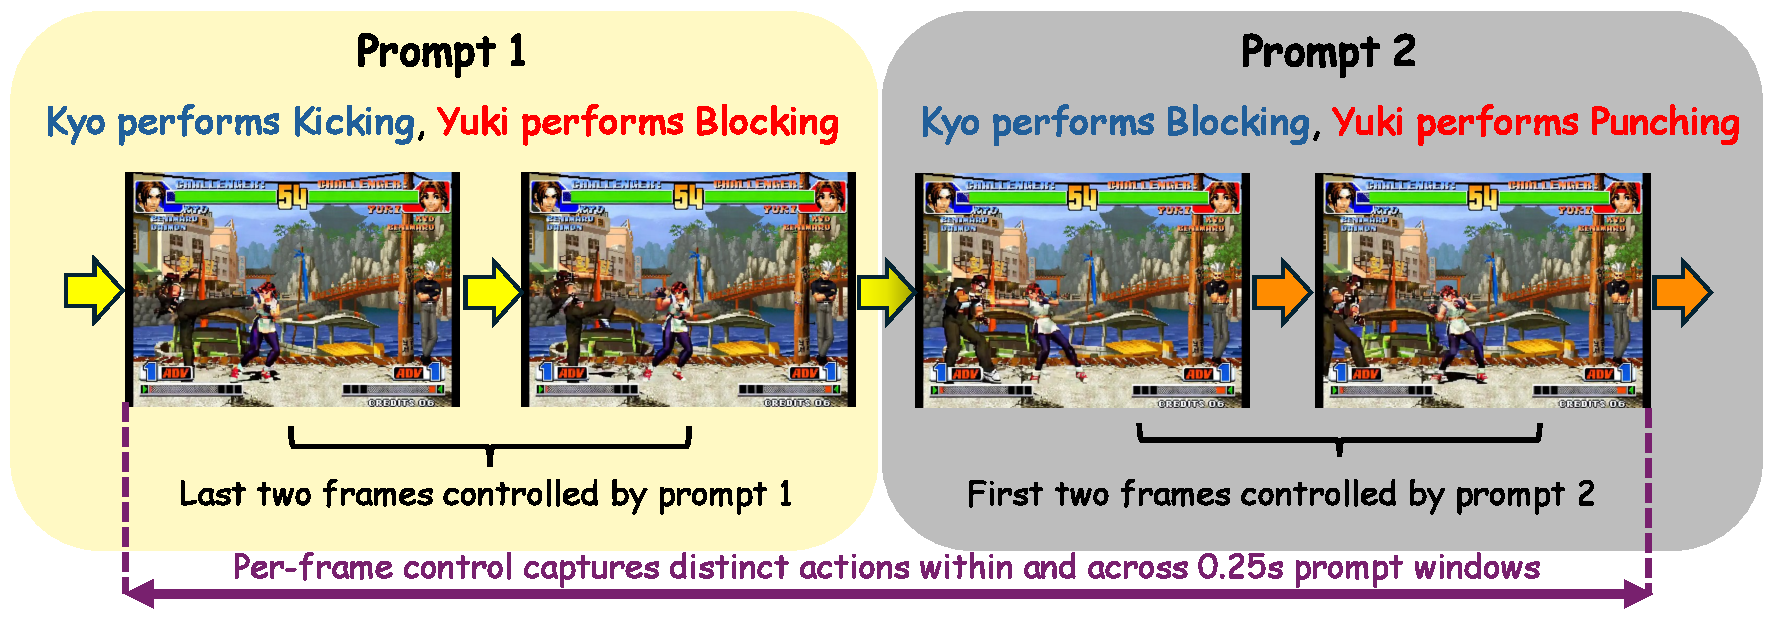
\includegraphics[width=\linewidth]{figures/kof.pdf}
    \caption{\textbf{Demonstrations of fine-grained multi-entity action control of \methodname in \textit{KOF}.}
    \methodname precisely responds to rapid action inputs and successfully captures
    actions as brief as $0.25$\,s (e.g., \textit{Punching}),
    demonstrating its fine-grained and responsive control capability.}
    \label{fig:kof_demo}
\end{figure*}
\paragraph{Action Interfaces of World Models.}
Existing world models inherit one of three action interfaces, each intrinsically limited
in generality and scalability across entities and worlds.
The first family encodes actions as \emph{engine-internal animation labels}, that is,
discrete identifiers exemplified by DIAMOND~\citep{alonso2024diffusion} on
Atari and Counter-Strike, where every index is bound at design time to a specific
in-game animation, leaving any out-of-vocabulary behavior inherently inexpressible.
The second family conditions generation on \emph{human-device inputs}, such as keyboard and mouse.
Representative systems include GameNGen~\citep{valevski2024diffusion},
the Genie series~\citep{bruce2024genie, parkerholder2024genie2, parkerholder2025genie3},
Oasis~\citep{oasis2024}, the Matrix-Game series~\citep{zhang2025matrixgame, he2025matrixgame2},
The Matrix~\citep{feng2024matrix}, MineWorld~\citep{guo2025mineworld},
WorldPlay~\citep{sun2025worldplay}, and GameFactory~\citep{yu2025gamefactory},
all of which condition on per-frame keyboard or mouse signals tied to a single player, so the schema cannot specify \emph{which} entity should act when
multiple entities co-exist within the scene.
The third family relies on \emph{scene-level captions}, where
GameGen-X~\citep{che2024gamegenx} feeds InstructNet with whole-clip multi-modal
instructions, Hunyuan-GameCraft-$2$~\citep{tang2025hunyuan} follows free-form prompts
such as ``open the door'', and LingBot-World~\citep{team2026advancing} further steers
global and local world events through textual prompts, each operating at the granularity
of the entire scene rather than any individual subject and thus conflating distinct
entities' behaviors under one global descriptor.
Across the three families, no prior interface simultaneously delivers open-vocabulary
semantics and per-entity addressability for independent simultaneous control of
multiple co-existing entities, exposing the core gap that our work targets.

% Early world models compressed game observations into compact latent spaces for planning~\citep{ha2018world, hafner2023mastering}.  The shift to diffusion-based rendering began with GameNGen~\citep{valevski2024diffusion} and DIAMOND~\citep{alonso2024diffusion}, which demonstrated real-time game generation on DOOM and Atari conditioned on single-entity low-level discrete actions.

% Early world models compressed game observations into compact latent spaces for planning~\citep{ha2018world, hafner2023mastering}. The shift to diffusion-based rendering began with GameNGen~\citep{valevski2024diffusion}, the first real-time diffusion game engine (DOOM, 20\,FPS), and DIAMOND~\citep{alonso2024diffusion}, which extended this to Atari. These systems are limited to single-entity discrete conditioning with no game-logic enforcement.
%%% NEW %%%
% Subsequent works have broadened the scope of game world modeling. GameGen-X~\citep{che2024gamegenx} and GameFactory~\citep{yu2025gamefactory} extend diffusion-based game generation to open-domain scenes with keyboard and mouse control. The Genie series~\citep{bruce2024genie, parkerholder2024genie2, parkerholder2025genie3} learns latent action representations from unlabeled video, enabling multi-minute 3D world generation. The Matrix~\citep{feng2024matrix} and Matrix-Game series~\citep{zhang2025matrixgame, he2025matrixgame2} scale to AAA-quality video at 16--25\,FPS for navigation and Minecraft scenarios, while WorldPlay~\citep{sun2025worldplay} and Infinite-World~\citep{wu2026infiniteworld} further advance streaming quality and long-horizon stability. Despite these improvements, all of these systems rely on low-level device inputs and are designed for a single operator, with no mechanism for independently commanding a second entity through a semantic vocabulary.
% GameGen-X~\citep{che2024gamegenx} and GameFactory~\citep{yu2025gamefactory} generalize diffusion-based game generation to open-domain scenes with keyboard/mouse action control, yet both remain single-player systems that operate with low-level input signals rather than semantic entity-level commands.

% More recent works have explored richer interaction modalities. Vid2World~\citep{huang2025vid2world} and Hunyuan-GameCraft-2~\citep{tang2025hunyuan} incorporate action-conditioned and instruction-following generation; AVID~\citep{rigter2024avid} and MineWorld~\citep{guo2025mineworld} adapt diffusion and autoregressive models for single-agent game generation; but all remain single-agent systems. Solaris~\citep{solaris2025} supports two players but generates \textit{independent} per-player streams from separate viewpoints, so mutual adversarial interaction within a shared scene is never jointly modeled. COMBAT~\citep{agarwal2026combat} learns reactive opponent behavior emergently from single-player fighting game data but offers no explicit interface to direct the opponent's strategy. MultiGen~\citep{po2026multigen} introduces multi-subject diffusion control via external memory but requires separate models per entity and is limited to first-person views. ShareVerse~\citep{zhu2026shareverse} and LiveWorld~\citep{duan2026liveworld} study multi-agent consistency in autonomous driving and persistent entity modeling respectively, but neither addresses interactive adversarial game combat with semantic control. LingBot-World~\citep{team2026advancing} combines text and keyboard inputs for long-horizon navigation but lack opponent modeling either.

% The Matrix~\citep{feng2024matrix} and the Matrix-Game series~\citep{zhang2025matrixgame, he2025matrixgame2} scale to AAA-quality video at 16--25\,FPS, but target open-world \emph{navigation} (ego-motion only) or Minecraft (WASD + mouse), both of which lack opponent modeling and episode-level game state. The Genie series~\citep{bruce2024genie, parkerholder2024genie2, parkerholder2025genie3} learns latent action representations from unlabeled video and achieves multi-minute 3D world generation, but accepts only raw keyboard/mouse inputs and provides no interface for independently commanding a second entity with a semantic vocabulary; they are \emph{world generators} rather than game engines.
% %%% NEW %%%
% WorldPlay~\citep{sun2025worldplay} and Infinite-World~\citep{wu2026infiniteworld} push streaming video world models to 720p/24\,FPS and 1000-frame horizons with long-term geometric consistency, but still accept only raw keyboard/mouse inputs with no multi-entity interface.
% Vid2World~\citep{huang2025vid2world} and Hunyuan-GameCraft-2~\citep{tang2025hunyuan} extend interactive world modeling to action-conditioned and instruction-following generation respectively, but both remain single-agent systems without independent opponent control.
% %%% NEW %%%
% AVID~\citep{rigter2024avid} adapts closed-source video diffusion models via learned masks without parameter access, and MineWorld~\citep{guo2025mineworld} replaces diffusion with a visual-action autoregressive Transformer for real-time Minecraft at 4--7\,FPS; both remain single-agent with no opponent modeling.
% Oasis~\citep{oasis2024} demonstrates real-time Minecraft generation. Solaris~\citep{solaris2025} extends this to two human players but generates \emph{independent} per-player streams from separate first-person viewpoints, so mutual adversarial interaction within a shared frame is never jointly modeled.
% COMBAT~\citep{agarwal2026combat} trains a 1.2\,B DiT world model on Tekken\,3 and learns reactive opponent behavior emergently from single-player data, but provides no explicit interface for independently commanding the opponent's strategy.
% MultiGen~\citep{po2026multigen} introduces external memory for editable diffusion game engines and symmetric real-time multiplayer rollouts, but only provides limited first-person views rather than full scenes and requires multiple models to control multiple subjects.
% ShareVerse~\citep{zhu2026shareverse} achieves multi-agent consistent video generation for shared-world autonomous driving, while LiveWorld~\citep{duan2026liveworld} models persistent entity evolution when unobserved; neither addresses interactive adversarial game combat with semantic control.
% LingBot-World~\citep{gao2026lingbotworld} achieves 16\,FPS long-horizon stability on navigation scenarios but provides only WASD/text control without opponent modeling.

% Across this landscape, our emphasis is different: in single-viewpoint multi-entity, long-horizon, cross-world settings, the conditioning interface is as much of a structural bottleneck as the generative backbone. Existing systems either rely on game-specific input conventions (keyboard and mouse, scene-level captions, or discrete action IDs), which inherit a particular operator-engine protocol, or on engine-internal animation namespaces, whose labels are entity-local and game-local. We instead adopt natural language as the conditioning interface: per-frame per-entity captioning yields a compositional unified action space along a \emph{namespace} facet (linear in entities, shared across games, open-vocabulary) and a \emph{token-decomposition} facet (entity-prefix and action-specific tokens recombinable at inference). To our knowledge, no prior video world model has provided independent per-frame natural language control of two heterogeneous entities sharing a single viewpoint, with the comparison summarized in \Cref{tab:comparison}.
% Our emphasis is different: in multi-entity, long-horizon, cross-world settings, the conditioning interface may be as much of a bottleneck as the generative backbone. Existing systems rely either on device-level inputs, which are tied to a single operator and one engine's input design, or on discrete action IDs, which share little structure across actions, entities, and worlds. We instead study natural language as the conditioning interface, because a single representation gives independent per-entity channels, semantic composition across entities, world-agnostic reuse, and pretrained semantic priors. To our knowledge, prior video world models do not provide independent per-frame semantic control of two heterogeneous entities within a shared adversarial viewpoint; Table~\ref{tab:comparison} summarizes the comparison.

% \begin{table}[t]
%   \caption{Systematic comparison of interactive video world models. \cmark~=~supported, \xmark~=~not supported, $\sim$~=~partial. \emph{Multi-entity} requires independent control of two entities with distinct action vocabularies. \emph{Semantic NL} requires per-frame natural language action descriptions.}
%   \label{tab:comparison}
%   \centering
%   \begin{tabular}{lcccc}
%     \toprule
%     Model & Multi-entity & Semantic NL & $\geq$16fps & $>$5min \\
%     \midrule
%     GameNGen~\citep{valevski2024diffusion}     & \xmark & \xmark & \cmark & \cmark \\
%     Genie~2~\citep{parkerholder2024genie2}     & $\sim$ & \xmark & \cmark & \xmark \\
%     Genie~3~\citep{parkerholder2025genie3}     & $\sim$ & \xmark & \cmark & $\sim$ \\
%     The Matrix~\citep{feng2024matrix}          & \xmark & \xmark & \cmark & \cmark \\
%     Matrix-Game 2.0~\citep{he2025matrixgame2}  & \xmark & \xmark & \cmark & $\sim$ \\
%     LingBot-World~\citep{team2026advancing}  & \xmark & \xmark & \cmark & \cmark \\
%     Solaris~\citep{solaris2025}                & \cmark & \xmark & $\sim$ & $\sim$ \\
%     \midrule
%     \textbf{\methodname (Ours)}                & \cmark & \cmark & \cmark & \cmark \\
%     \bottomrule
%   \end{tabular}
% \end{table}

% \paragraph{Efficient Streaming Video Generation. }
% Several lines of work advance streaming video generation from complementary angles.
% On the diffusion side, Flow Matching~\citep{lipman2022flow} and Distribution Matching Distillation (DMD)~\citep{yin2024one} substantially reduce the number of inference steps.
% On the autoregressive side, Self-Forcing~\citep{chen2025selfforcing} eliminates exposure bias caused by the training-inference discrepancy.
% For long-horizon memory management, StreamingLLM~\citep{xiao2023streamingllm} and LM-Infinite~\citep{han2023lminfinite} bound memory usage via attention-sink tokens and sliding-window KV caches.
% Our work integrates these advances together to achieve real-time long-horizon streaming generation.

% Self-Forcing~\citep{chen2025selfforcing} eliminates exposure bias for autoregressive video generation. StreamingLLM~\citep{xiao2023streamingllm} and LM-Infinite~\citep{han2023lminfinite} introduce attention-sink tokens and sliding-window KV caches to bound memory in language models while keeping position indices within a trained range. Flow matching~\citep{lipman2022flow} and consistency distillation~\citep{song2023consistency} reduce diffusion inference steps. Our RoPE-decoupled KV-cache sliding adapts the attention-sink principle to autoregressive video diffusion under two constraints absent from language settings: keys must be stored \emph{pre-rotation} so that local positions can be reassigned on-the-fly without cache invalidation, and the sliding window size is calibrated to the typical duration of an entity-level action rather than to linguistic context length. Together, these adaptations yield the first streaming method to jointly address memory boundedness, positional OOD prevention, and real-time throughput in an interactive video world model.
